
\begin{figure}[H]
  \centering
  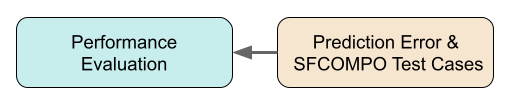
\includegraphics[width=0.7\linewidth]{./chapters/exp1/methodology4.png}
  \caption{Fourth portion of the flowchart from Figure \ref{fig:method} being 
           described in this section.}
\end{figure}

\subsection{Random Error Impacts on Prediction}
\label{sec:randerr}

As previously introduced in Section \ref{sec:testerr}, the prediction errors
are compared among the three approaches to understand the performance.

Error metrics being used, implementation details (not really any, just python scripts)

Conf matrix, ROC Curve, Learning curve (Maybe for 1\% and 10\% error cases?)

\begin{figure}[!ht]
    \centering
    \begin{subfigure}[b]{0.49\textwidth}
        \centering
        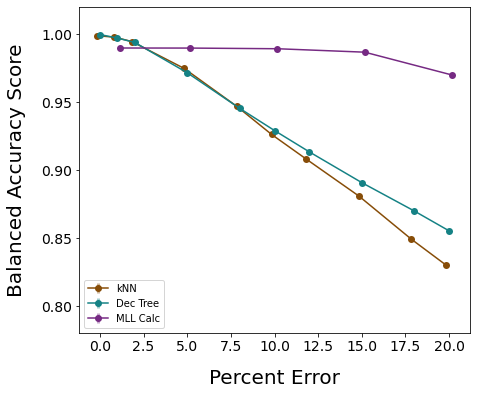
\includegraphics[width=\textwidth]{./chapters/exp1/randerr_compare_nuc29_BalAcc_rxtr.png}
        \caption[]{Caption.}
        %\label{fig:}
    \end{subfigure}
    \hfill
    \begin{subfigure}[b]{0.49\textwidth}
        \centering
        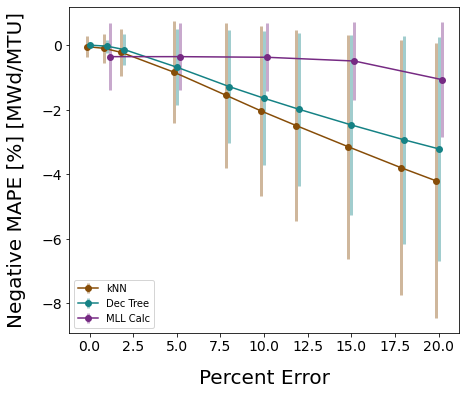
\includegraphics[width=\textwidth]{./chapters/exp1/randerr_compare_nuc29_MAPE_burn.png}
        \caption[]{Caption.}
        %\label{fig:}
    \end{subfigure}
    \vskip\baselineskip
    \begin{subfigure}[b]{0.49\textwidth}
        \centering
        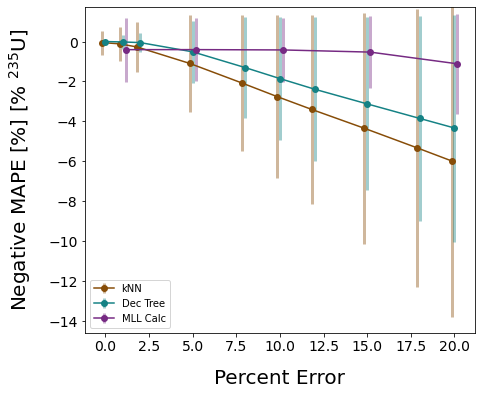
\includegraphics[width=\textwidth]{./chapters/exp1/randerr_compare_nuc29_MAPE_enri.png}
        \caption[]{Caption.}
        %\label{fig:}
    \end{subfigure}
    \hfill
    \begin{subfigure}[b]{0.49\textwidth}
        \centering
        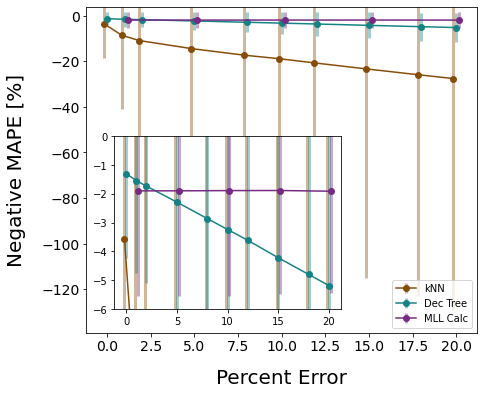
\includegraphics[width=\textwidth]{./chapters/exp1/randerr_compare_nuc29_MAPE_cool.png}
        \caption[]{Caption.}
        %\label{fig:}
    \end{subfigure}
    \caption[]{Caption Caption.}
    %\label{fig:}
\end{figure}

\begin{figure}[!ht]
    \centering
    \begin{subfigure}[b]{0.49\textwidth}
        \centering
        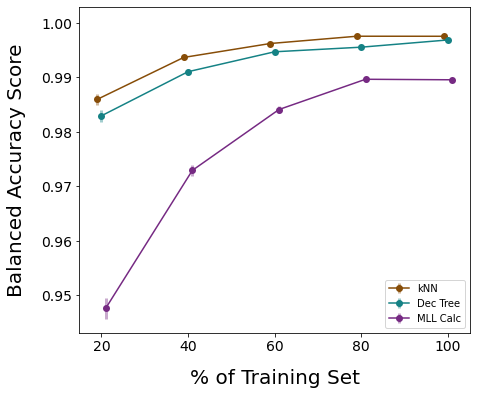
\includegraphics[width=\textwidth]{./chapters/exp1/learncurve_nuc29_BalAcc_rxtr.png}
        \caption[]{Caption.}
        %\label{fig:}
    \end{subfigure}
    \hfill
    \begin{subfigure}[b]{0.49\textwidth}
        \centering
        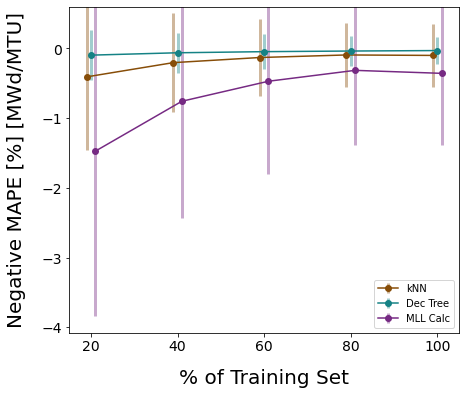
\includegraphics[width=\textwidth]{./chapters/exp1/learncurve_nuc29_MAPE_burn.png}
        \caption[]{Caption.}
        %\label{fig:}
    \end{subfigure}
    \vskip\baselineskip
    \begin{subfigure}[b]{0.49\textwidth}
        \centering
        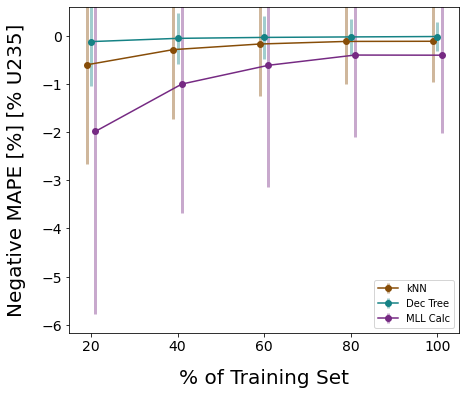
\includegraphics[width=\textwidth]{./chapters/exp1/learncurve_nuc29_MAPE_enri.png}
        \caption[]{Caption.}
        %\label{fig:}
    \end{subfigure}
    \hfill
    \begin{subfigure}[b]{0.49\textwidth}
        \centering
        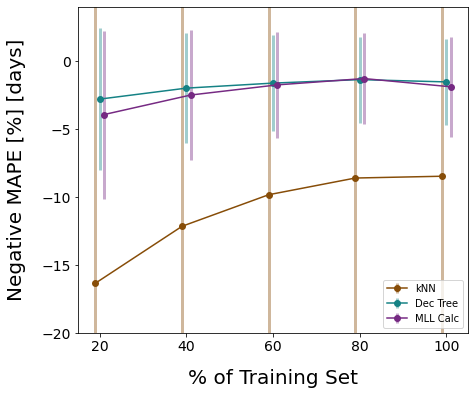
\includegraphics[width=\textwidth]{./chapters/exp1/learncurve_nuc29_MAPE_cool.png}
        \caption[]{Caption.}
        %\label{fig:}
    \end{subfigure}
    \caption[]{Caption Caption.}
    %\label{fig:}
\end{figure}

\begin{figure}[!ht]
  \centering
  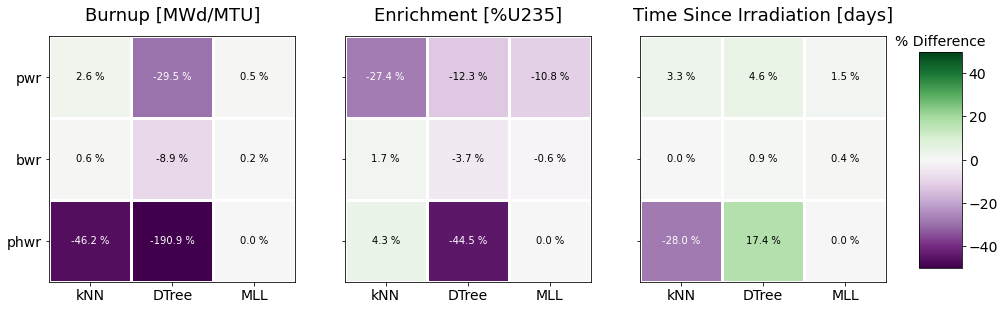
\includegraphics[width=1.1\textwidth]{./chapters/exp1/rxtr-type_known-unknown_diff.png}
  \caption{diff.}
  \label{fig:knownrxtr}
\end{figure}

\subsection{SFCOMPO Test Set}
\label{sec:sfcompo}

The testing described in Section \ref{sec:randerr} describes the process of
evaluating the methodology with test cases drawn from the training database.
It is also helpful to test the methodology against real assays of \gls{SNF}.
The \gls{SFCOMPO} database was created to allow access to these sorts of
measurements linked to the reactor operation parameters being predicted in this
work. The only parameter not part of the \gls{SFCOMPO} database is the time
since irradiation, so that is not predicted here. 

There are 505 test cases that are able to be compared against the training
database.  The number of each reactor type is as follows: 312 \gls{PWR}s, 165
\gls{BWR}s, and 28 \gls{PHWR}s. The space of enrichment and burnup values is
visualized in Figure \ref{fig:sfcoscatter}. These are sufficienty represented
in the training set design, as pictured in Figure \ref{fig:trainhist}.

\begin{figure}[!ht]
    \centering
    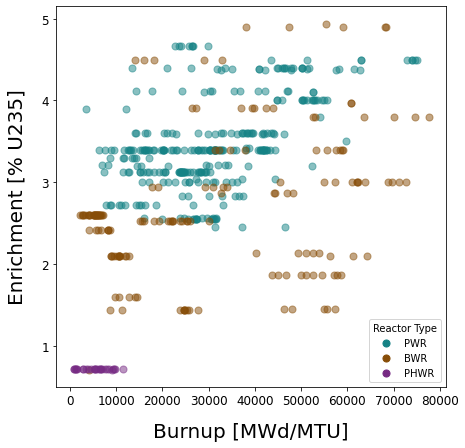
\includegraphics[width=0.7\textwidth]{./chapters/exp1/sfcompo_scatter_viz.png}
    \caption{Scatter plot showing the range of reactor operation parameters in 
             the \gls{SFCOMPO} testing set that are being predicted.}
    \label{fig:sfcoscatter}
    \todo[inline]{increase tick size, change order to bwr, pwr, phwr. Maybe show 
                  comparison against training E v B scatter plot}
\end{figure}



\begin{table}[!ht]
  \centering
  \begin{tabular}{@{}l|lll|lll@{}}
  \toprule
                   & \multicolumn{3}{l|}{Accuracy Scores} & \multicolumn{3}{l}{Balanced Accuracy Scores} \\ \toprule
  Null Handling    & kNN        & DTree      & MLL       & kNN           & DTree         & MLL           \\ \midrule
  Imputed Nulls    & 0.52       & 0.60       & 0.39      & 0.09          & 0.12          & 0.00          \\
  Zero-value Nulls & 0.45       & 0.42       & 0.72      & 0.21          & 0.30          & 0.63          \\ \bottomrule
  \end{tabular}
  \caption{sfcompo reactor accuracies.}
  \label{tbl:sfcorxtr}
\end{table}

\begin{figure}[!ht]
    \centering
    \begin{subfigure}[b]{0.49\textwidth}
        \centering
        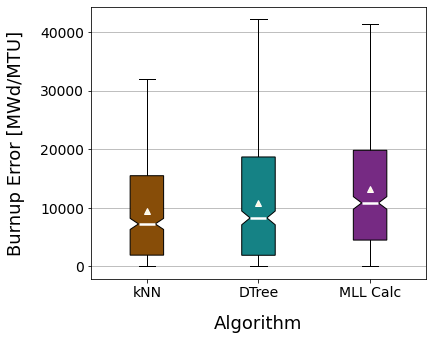
\includegraphics[width=\textwidth]{./chapters/exp1/sfcompo_boxplots_impnull_burn.png}
        \caption[]{Caption.}
        %\label{fig:}
    \end{subfigure}
    \hfill
    \begin{subfigure}[b]{0.49\textwidth}
        \centering
        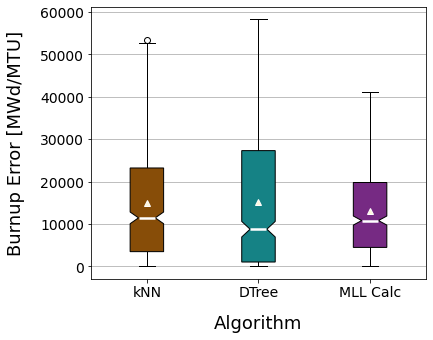
\includegraphics[width=\textwidth]{./chapters/exp1/sfcompo_boxplots_0null_burn.png}
        \caption[]{Caption.}
        %\label{fig:}
    \end{subfigure}
    \caption{sfcompo burnup boxplots.}
    \label{fig:sfcoburn}
\end{figure}

\begin{table}[!ht]
  \centering
  \begin{tabular}{@{}l|lll|lll@{}}
  \toprule
                   & \multicolumn{3}{l|}{Mean Errors [GWd/MTU]} & \multicolumn{3}{l}{Median Errors [GWd/MTU]} \\ \toprule
  Null Handling    & kNN           & DTree         & MLL           & kNN            & DTree          & MLL    \\ \midrule
  Imputed Nulls    & 9.43          & 10.89         & 13.17         & 7.26           & 8.28           & 10.84  \\
  Zero-value Nulls & 14.88         & 15.18         & 3.53          & 11.47          & 8.79           & 1.70   \\ \bottomrule
  \end{tabular}
  \caption{sfcompo burnup errors.}
  \label{tbl:sfcoburn}
\end{table}

\begin{figure}[!ht]
    \centering
    \begin{subfigure}[b]{0.49\textwidth}
        \centering
        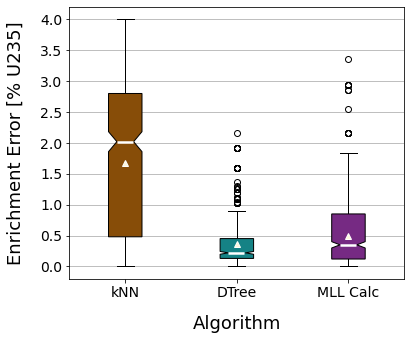
\includegraphics[width=\textwidth]{./chapters/exp1/sfcompo_boxplots_0null_enri.png}
        \caption[]{Caption.}
        %\label{fig:}
    \end{subfigure}
    \hfill
    \begin{subfigure}[b]{0.49\textwidth}
        \centering
        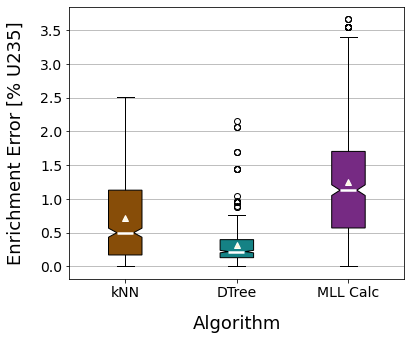
\includegraphics[width=\textwidth]{./chapters/exp1/sfcompo_boxplots_impnull_enri.png}
        \caption[]{Caption.}
        %\label{fig:}
    \end{subfigure}
    \caption{sfcompo enrichment boxplots.}
    \label{fig:sfcoenri}
\end{figure}

\begin{table}[!ht]
  \centering
  \begin{tabular}{@{}l|lll|lll@{}}
  \toprule
                   & \multicolumn{3}{l|}{Mean Errors [\% U235]} & \multicolumn{3}{l}{Median Errors [\% U235]} \\ \toprule
  Null Handling    & kNN           & DTree          & MLL          & kNN            & DTree          & MLL    \\ \midrule
  Imputed Nulls    & 0.72          & 0.31           & 1.25         & 0.50           & 0.22           & 1.13   \\
  Zero-value Nulls & 1.67          & 0.36           & 0.49         & 2.02           & 0.22           & 0.35   \\ \bottomrule
  \end{tabular}
  \caption{sfcompo enrichment errors.}
  \label{tbl:sfcoenri}
\end{table}

